\documentclass[twocolumn,10pt,a4paper]{article}
\usepackage[margin=0.75in]{geometry}
\usepackage[utf8]{inputenc}
\usepackage[T1]{fontenc}
\usepackage{lmodern}
\usepackage{microtype}
\usepackage{cite}
\usepackage{url}
\usepackage{hyperref}
\usepackage{xcolor}
\usepackage{enumitem}
\usepackage{tabularx}
\usepackage{booktabs}
\usepackage{graphicx}
\hypersetup{colorlinks=true,citecolor=blue,linkcolor=blue,urlcolor=blue}

\title{A Closed-Loop Day-2 Remediation Architecture for O-RAN Cloud Infrastructure Using Standardized Interfaces}

\author{David Kypuros \\
\small Red Hat \\
\small \texttt{dkypuros@redhat.com}}

\date{31 May 2026}

\begin{document}
\maketitle

\begin{abstract}
This paper describes a closed-loop Day-2 remediation pattern for O-RAN Cloud RAN deployments. The pattern composes four published interface contracts: the O-RAN O2 Infrastructure Management Services (O2 IMS) API as the SMO-to-O-Cloud provisioning surface; Kubernetes-native Custom Resource Definitions (Metal3 BareMetalHost / HostFirmwareComponents, Machine Config Operator, Kernel Module Management) as the delivery substrate; TM Forum TMF688 and TMF921 as the audit and intent envelopes; and IEEE 1588 / O-RAN WG6 Cloud Notifications as the timing-domain observation contract. We claim the novelty lies in the conjunction of O2 General Aspects and Principles, O2 IMS Interface, Metal3, and Machine Config Operator under a single deterministic routing rule that classifies infrastructure faults against the O-RAN WG6 O-Cloud resource model before any large language model is consulted. The contribution extends a prior multivendor diagnostic substrate by closing the loop from fault to audited remediation through a five-gate guardrail and a digital twin pass. The runtime is open-source and shipped with a verify gate that produces a binary pass/fail any reviewer can reproduce. We acknowledge that v0 runtime is stub-driven and that production wiring is future work.
\end{abstract}

\section{Introduction}

Day-2 operations on a multivendor Cloud RAN deployment span a wide functional surface: timing drift on a worker node, firmware regressions on accelerator NICs, host service interference with the PTP hardware clock, driver swaps for fixed-function offloads, configuration churn from upstream SMO intents. Each of these is observable, each has an audited path to remediation, and yet the bridges between diagnosis and execution are uneven across vendors and standards bodies.

Prior agentic-AI work for RAN automation has clustered around two failure modes. The first stops at the SMO boundary: an agent converges on a root cause and emits an intent, but the intent never crosses into a concrete delivery contract. The second invents a parallel controller plane that side-steps O-RAN's own resource layering, which is operationally fragile and politically expensive in a multivendor ecosystem. A prior multivendor diagnostic publication established a fault-localization substrate for Cloud RAN troubleshooting \cite{multivendor_blog_2026} but left the loop open: the diagnostic agents converge on a root cause and emit an artifact, while the actual remediation path remains undefined.

This paper closes the loop. We describe a harness pattern that takes the diagnostic artifact as input, classifies it against a deterministic taxonomy grounded in the O-RAN O-Cloud resource model \cite{oran_wg1_arch,oran_o2_ganp}, routes the resulting proposal through the O-RAN O2 IMS interface \cite{oran_o2_ims} into Kubernetes-native CRD contracts \cite{metal3_bmo,openshift_mco,kmm_operator}, and emits a TM Forum TMF688 audit envelope \cite{tmf688} with an embedded reversibility profile before any apply is authorized. The four pieces (observation loop, cognitive middle, routing decision, sandbox plus operator seam) are described in order. The architectural novelty is the simultaneous conjunction of references \cite{oran_o2_ganp}, \cite{oran_o2_ims}, \cite{metal3_bmo}, and \cite{openshift_mco}, which we will refer to as the 2+3+8+9 conjunction following the bibliography numbering of the source repository.

The remainder of the paper is organized as follows. Section \ref{sec:background} establishes the standards and project context for each interface composed. Section \ref{sec:arch} describes the architecture in three logical pieces. Section \ref{sec:proto} summarizes the prototype, the five committed walkthrough scenarios, and the verify gate. Section \ref{sec:discuss} discusses positioning against adjacent projects and the standards-track ask. Section \ref{sec:conclude} concludes.

\section{Background}
\label{sec:background}

\textbf{O-RAN architecture and the O-Cloud surface.} The O-RAN Alliance Working Group 1 architecture description \cite{oran_wg1_arch} and Working Group 6 O2 General Aspects and Principles \cite{oran_o2_ganp} jointly define the O-Cloud resource model and the SMO-to-O-Cloud interface family. The O2 IMS specification \cite{oran_o2_ims} carries the infrastructure provisioning request and response envelopes; O2 DMS \cite{oran_o2_dms} carries deployment management. This work targets O2 IMS exclusively: the harness handles infrastructure remediation, not deployment lifecycle. The reference O2 IMS implementation cited throughout is Red Hat's open-source O-Cloud Manager \cite{oran_o2ims_ocm}. The Decoupled SMO Architecture technical report \cite{oran_decoupled_smo} introduces the SMO Service (SMOS) abstraction, into which a closed-loop remediation harness fits naturally as a candidate first-class SMOS.

\textbf{Delivery substrate.} Below the O2 IMS interface, three Kubernetes-native operators carry the actual change: the Machine Config Operator \cite{openshift_mco} for host configuration, the Kernel Module Management Operator \cite{kmm_operator} for driver swaps, and Metal3 \cite{metal3_project,metal3_bmo} for bare-metal firmware and provisioning. Out-of-band firmware writes pass through the host BMC via DMTF Redfish \cite{dmtf_redfish}.

\textbf{Timing and observation.} The PTP stack on each worker uses linuxptp \cite{linuxptp_ptp4l} to discipline the PTP Hardware Clock (PHC) against an upstream Grandmaster, conforming to IEEE 1588-2019 \cite{ieee_1588_2019} and the ITU-T G.8275.1 telecom profile \cite{itu_g82751}. The Red Hat PTP Operator \cite{redhat_ptp_operator} orchestrates linuxptp on the cluster, and the cloud-event-proxy sidecar \cite{cloud_event_proxy} publishes state transitions as CloudEvents \cite{cncf_cloudevents} carrying the O-RAN WG6 Cloud Notifications payload \cite{oran_cloud_notifications}. The harness consumes that notification envelope as the inbound fault contract.

\textbf{Audit and intent.} TM Forum TMF688 \cite{tmf688} provides the event-management envelope used as the audit sink. TMF921 \cite{tmf921} provides the intent management envelope used for the dual-route notification path from the harness to the partner SMO. The SID information framework \cite{tmf_gb922} grounds the conceptual model that maps O-RAN resource classes to TM Forum entity types.

\section{System Architecture}
\label{sec:arch}

\begin{figure*}[t]
\centering
\includegraphics[width=0.95\textwidth]{../talk/architecture.png}
\caption{Seven-component macro architecture. The left side carries the observation loop (PTP Operator, cloud-event-proxy, O-RAN WG6 Cloud Notifications). The center carries the Agent Harness (Agentic Gateway plus four MCP servers plus three domain agents plus the deterministic Router). The right side forks: UP via TMF921 to the partner SMO, DOWN via O2 IMS to the O-Cloud. The Digital Twin substrate sits beneath the harness; the Killswitch is a global override above it.}
\label{fig:arch_macro}
\end{figure*}

The architecture has three logical pieces and an overhead control: the left loop (observation), the cognitive middle, the right loop (routing and delivery), and the Killswitch as a global override. Figure~\ref{fig:arch_macro} shows the macro layout.

\subsection{Left loop: observation}

Telemetry originates in the timing domain. Each Cloud RAN worker runs a PTP Hardware Clock disciplined by linuxptp daemons (\texttt{ptp4l} and \texttt{phc2sys}) \cite{linuxptp_ptp4l}, conforming to IEEE 1588-2019 \cite{ieee_1588_2019} and the G.8275.1 telecom profile \cite{itu_g82751}. The PTP Operator \cite{redhat_ptp_operator} runs the daemons and the cloud-event-proxy sidecar \cite{cloud_event_proxy} watches their state transitions. When the daemon state crosses a threshold (SYNCHRONIZED to HOLDOVER, master offset spike, monotonic PHC drift), the sidecar emits a CloudEvent \cite{cncf_cloudevents} with the O-RAN WG6 Cloud Notifications payload \cite{oran_cloud_notifications}.

The harness consumes this envelope as a \texttt{FaultPayload} (a JSON Schema draft-07 contract carried at \texttt{harness/schemas/FaultPayload.json}). The repository's scenario \texttt{D\_phc\_drift\_hw\_only} demonstrates the canonical divergence pattern that gives the harness its diagnostic edge: \texttt{ptp4l} reports SYNCHRONIZED (software view of the timing chain is healthy) while \texttt{phc2sys} reports monotonic frequency drift in parts-per-billion and the NIC reports rising \texttt{tx\_hwtstamp\_timeouts} (hardware view is not healthy). A purely software-layer observer would miss this; the harness reads both.

\subsection{Cognitive middle}

The Agentic Gateway terminates the CloudEvents stream and presents vendor-private tooling to the agent runtime under controlled MCP interfaces \cite{mcp_spec,mcp_python_sdk,fastmcp}. Four FastMCP servers run behind the gateway: \texttt{mcp-platform} (linuxptp daemons, host services, driver versions, NIC counters), \texttt{mcp-ran} (cell sync, PM counters, RAN parameters), \texttt{mcp-hardware} (NIC PHC introspection, BMC Redfish, CPU performance counters), and \texttt{mcp-ocloud} (the O-Cloud Manager inventory and alarms). The architectural pattern describes mTLS, OAuth2, and IP allowlist as the production posture; the v0 lab trusts localhost.

Three domain agents (Platform, RAN, Hardware) consume the MCP surface and converge on a root cause artifact (RCA). The cognitive middle's deterministic core is the Remediation Router. The router consults a 20-entry taxonomy declared in \texttt{harness/taxonomy.yaml} that maps every fault class onto the O-RAN WG6 O-Cloud resource model. The taxonomy carries an explicit grounding disclaimer in its first eighteen lines: the 20 subtypes are interpretive mappings within the three normative resource classes from O2-GAnP Figure 3.4-1 (Physical Resource, Logical Resource, Managed O-Cloud Service), not extensions to the spec.

The deterministic taxonomy lookup fires first; an LLM is consulted only when the result is the \texttt{ambiguous} class. This ordering is enforced in code and proven by the test suite. The repository's \texttt{contribution-1-routing-rule.yaml} declares the rule, the runtime at \texttt{harness/runtime/router.py} implements it, and the test \texttt{test\_route\_ambiguous\_with\_llm\_mode\_live} demonstrates that the LLM seam is wired through without becoming load-bearing on the routing decision.

\subsection{Right loop: routing and dual-route delivery}

The routing decision splits along the O-RAN resource-layer boundary. \textbf{Service-layer} faults (cell re-home, RAN parameter changes, slice intent updates, vDU software version rollouts) belong to the partner SMO. The harness does not execute them; it emits a TMF921 intent \cite{tmf921} and observes the dispatch result. This is the up route.

\textbf{Infrastructure-layer} faults go down through the O2 IMS interface \cite{oran_o2_ganp,oran_o2_ims} into the O-Cloud Manager \cite{oran_o2ims_ocm}, which dispatches into one of three reconcilers: Machine Config Operator \cite{openshift_mco} for host configuration changes, KMM \cite{kmm_operator} for driver swaps, Metal3 BMO \cite{metal3_bmo} for node firmware. Firmware writes pass through the host BMC via DMTF Redfish UpdateService.SimpleUpdate \cite{dmtf_redfish}. This is the down route. In the v0 implementation, the down route is a real Python function call from the router into a stubbed O-Cloud Manager that returns a shape-correct \texttt{o2ims\_dispatch} envelope; the envelope is attached to the audit so the operator sees the O2 IMS hop as a row in the record, not as a synthesized path string.

The dual-route pattern fires both branches simultaneously when an infrastructure action carries inherent service-layer impact. Scenario \texttt{E\_nic\_firmware\_update} is the teaching case: a NIC firmware update via Metal3 takes the host offline for a reboot window, so the harness emits a TMF921 companion intent up to the partner SMO in parallel with the O2 IMS down-route apply. The partner SMO's response (acceptance or rejection) lands on the audit's \texttt{dispatch\_result} field before operator co-authorization. Scenario \texttt{E\_with\_smo\_reject} demonstrates the rejection path: same down-route verdict, SMO rejects the maintenance window because neighboring cells are at 92 percent capacity. The operator sees both outcomes and is the reconciliation point.

\subsection{Sandbox gate and reversibility}

Before any apply, the proposal traverses a deterministic five-gate guardrail engine declared at \texttt{harness/guardrails.yaml} and executed at \texttt{harness/runtime/guardrail.py}. The gates fire in order: crisis\_mode global override, sandbox apply\_allowed (verdict produced by the Twin pass), action\_allowlist, blast\_radius caps (one node, one site, four cells in v0), and requiresHumanApproval. The Sandbox stage is operationally flexible: a same-topology mirrored cluster or a simulated linuxptp plus NIC driver stack satisfies the contract.

Every audit event carries a populated \texttt{ReversibilityProfile} with seven fields: rollback intent, blast-radius-if-reverse, rebuild timeline, replication history, validation history, risk profile burn-down, and confidence in reversibility. The intent is that the operator has the rollback contract at decision time, not after-the-fact. Figure~\ref{fig:governance} shows the governance layer in detail.

\begin{figure}[t]
\centering
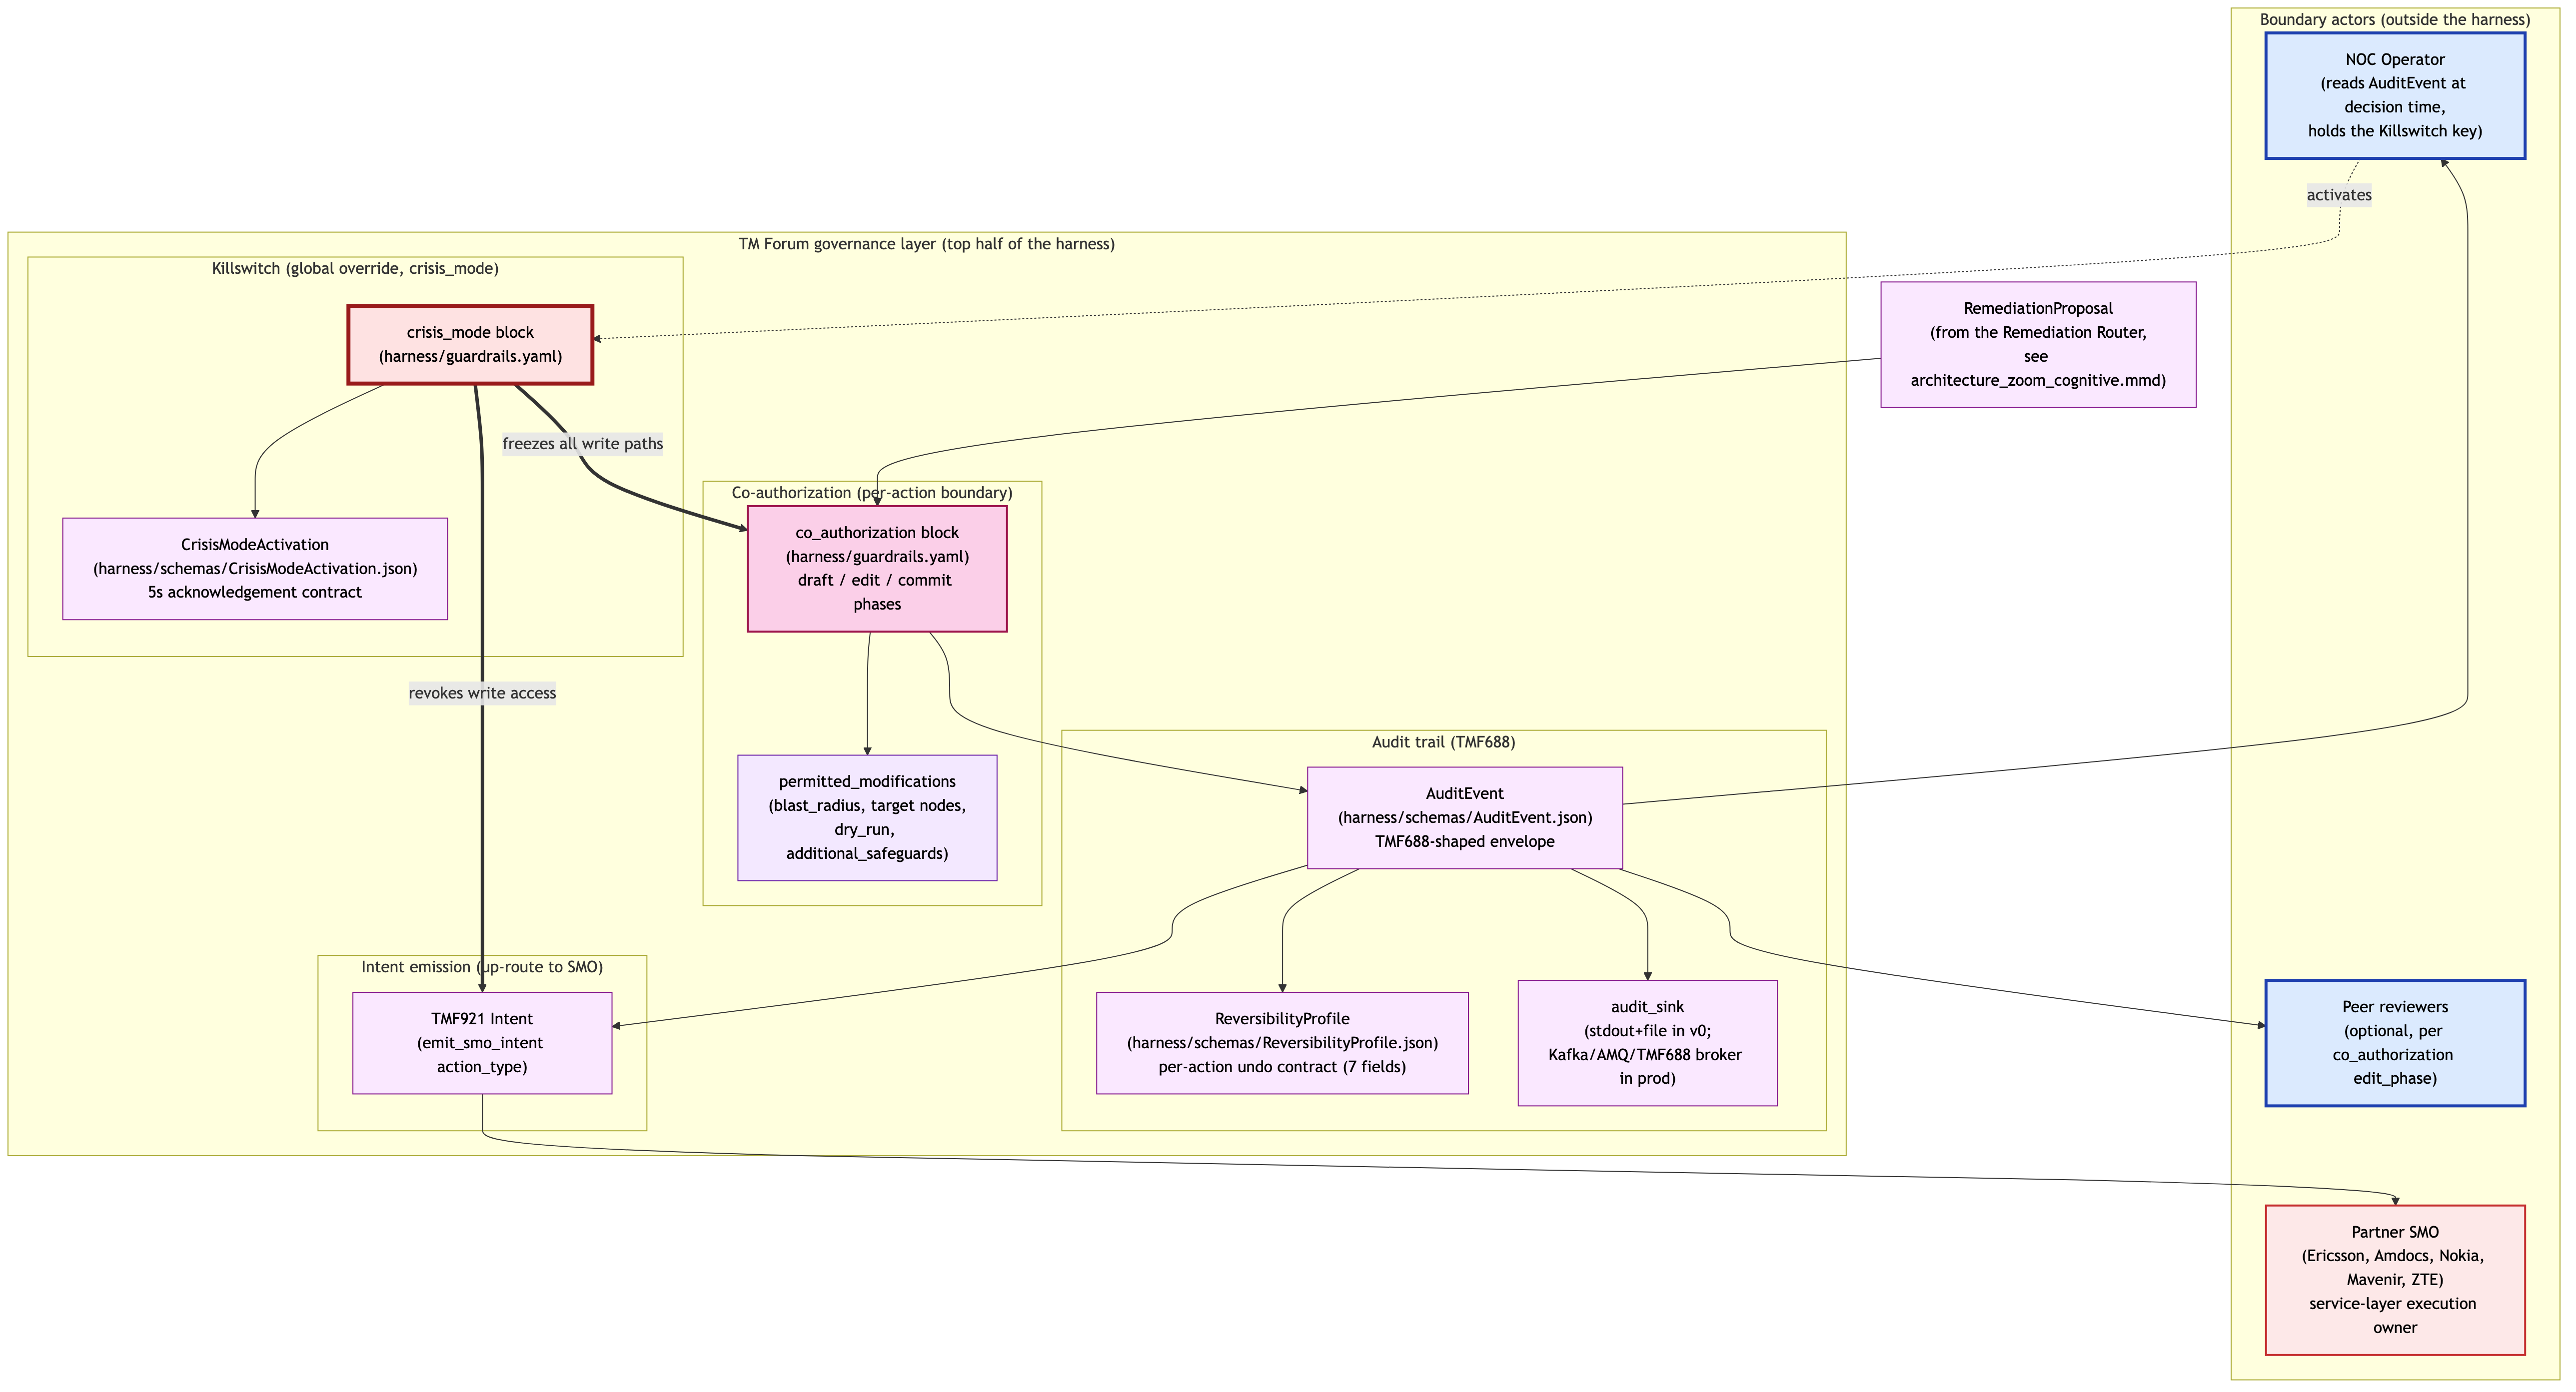
\includegraphics[width=\columnwidth]{../talk/architecture_zoom_governance.png}
\caption{Governance layer zoom. The TMF688 audit event carries the proposal, the guardrail result, the sandbox verdict, the optional companion intent with its dispatch result, and the seven-field ReversibilityProfile. The co-authorization contract sits between draft and commit. The Killswitch (crisis\_mode) is the global override.}
\label{fig:governance}
\end{figure}

\subsection{Killswitch as global override}

A \texttt{crisis\_mode} flag in \texttt{guardrails.yaml} is the global override. When activated by a NOC supervisor in response to a macro event (storms, security incidents, regional outages), all write paths revoke, EvalOps confidence pins to zero, and telemetry routes to a manual queue. The Reversibility Profile rewinds one applied action; the Killswitch freezes all of them. The two compose.

\section{Prototype and Walkthroughs}
\label{sec:proto}

\begin{figure}[t]
\centering
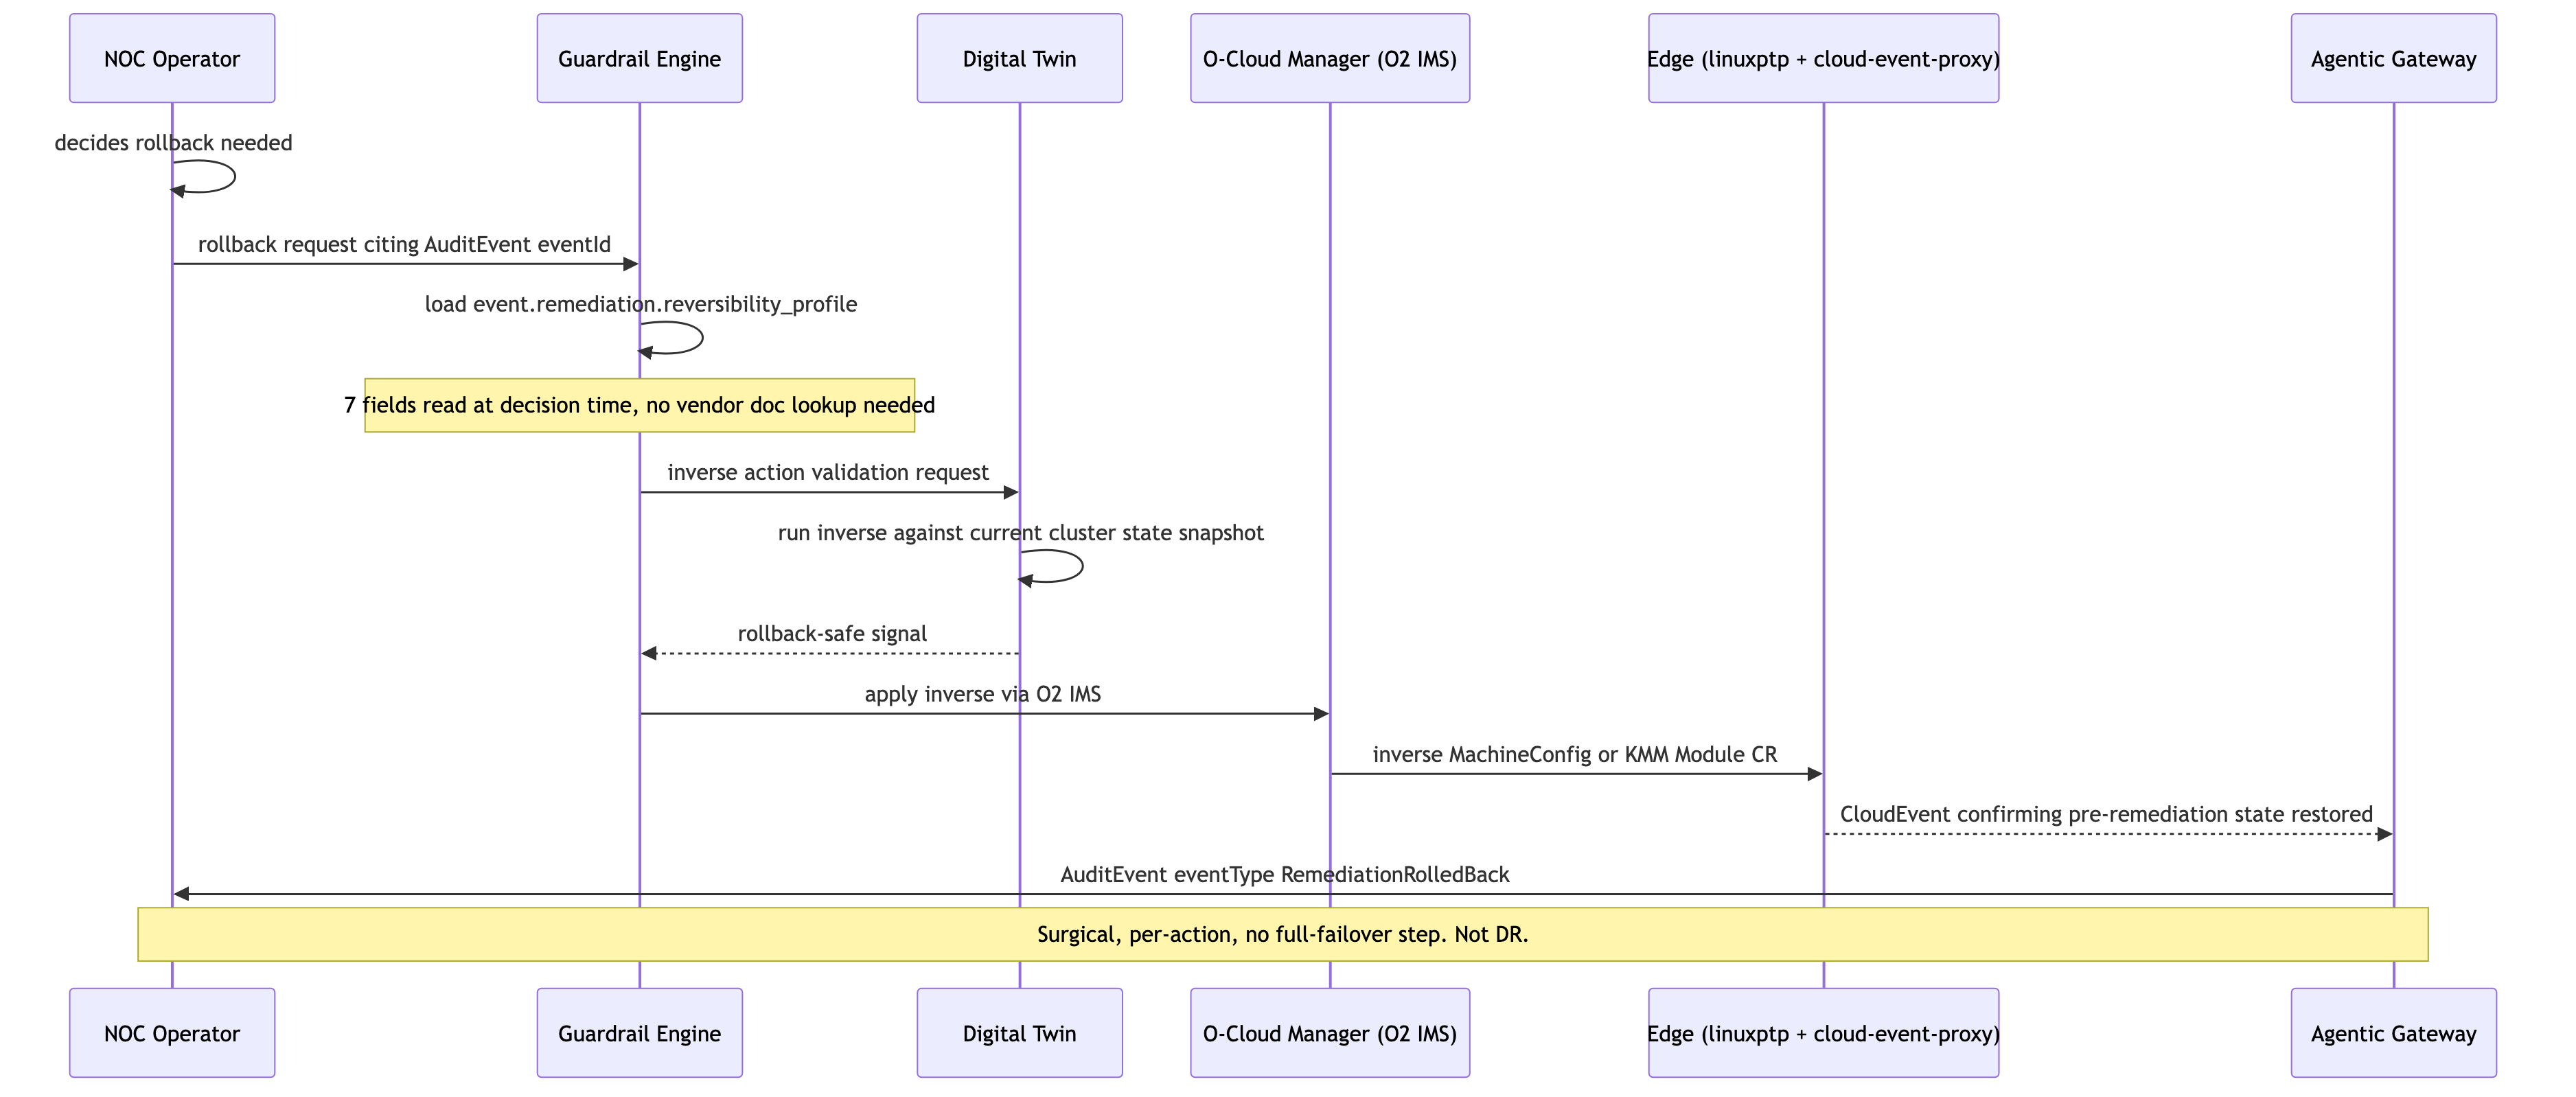
\includegraphics[width=\columnwidth]{../talk/sequence_agentic_recovery.png}
\caption{Sequence diagram for a single closed-loop remediation cycle. PTP CloudEvent arrives at the gateway, traverses the cognitive middle to a RemediationProposal, passes the sandbox apply-allowed gate and the five-gate guardrail, lands on the operator's co-authorization seat, and emits a TMF688 audit event with the reversibility profile attached.}
\label{fig:sequence}
\end{figure}

The repository ships five end-to-end fixture scenarios under \texttt{scenarios/}: \texttt{A\_fw\_lldp\_agent} (a host service interfering with PTP, routed to MCO), \texttt{A\_prime\_ice\_driver} (an outdated NIC driver causing PHC drift, routed to KMM), \texttt{D\_phc\_drift\_hw\_only} (the hardware-only divergence demonstrating the diagnostic edge), \texttt{E\_nic\_firmware\_update} (the dual-route firmware case with accepted companion intent), and \texttt{E\_with\_smo\_reject} (the same firmware path with a rejected companion intent). Each scenario carries a \texttt{fault\_payload.json} input, a remediation YAML, and a committed \texttt{audit\_event.json} fixture that the verify gate replays against the actual walker output.

The runtime pipeline (walker, router, sandbox, guardrail) is deterministic. A reviewer can clone the repository, install only PyYAML and jsonschema, and run \texttt{python3 scripts/verify.py}. The gate completes ten checks in under five seconds: citation header completeness on every authored YAML and JSON, JSON and YAML parse, conformance-table bidirectional completeness, an em-dash audit, a leakage guard, README structural sanity, file counts, JSON Schema validation of every scenario artifact, and end-to-end walker replay against committed audit fixtures on seven material fields. The reference state in the repository at the time of writing reports ten of ten checks pass.

\section{Discussion}
\label{sec:discuss}

\textbf{The 2+3+8+9 novelty conjunction.} The architecture's central claim is that a single \texttt{RemediationProposal} travels through the O2 IMS contract surface \cite{oran_o2_ganp,oran_o2_ims} and lands at a Kubernetes-native CRD reconciler \cite{metal3_bmo,openshift_mco} without a custom controller plane in between. The conjunction of these four references is not a re-derivation of prior architectures; existing agentic-RAN work either stops at the SMO boundary without a delivery story, or proposes a parallel controller plane. The harness pattern composes existing contracts.

\textbf{Comparison to ONAP, Nephio, OSM.} ONAP \cite{onap}, Nephio \cite{nephio}, and Open Source MANO \cite{osm} are orchestration platforms that manage network function lifecycle at scale. The harness pattern is closed-loop remediation: fault-driven cognition that emits a proposal, gates it, audits it, and observes the operator's commit. The two compose. Nephio can deliver the standing topology; the harness handles post-deployment Day-2 anomalies on top of that topology.

\textbf{Positioning against the Decoupled SMO Architecture.} The closed-loop harness fits the SMOS abstraction described in WG1 TR R004 \cite{oran_decoupled_smo}. It exposes a TMF688 audit surface and a TMF921 intent surface, both SMOS-compatible by construction. A reasonable standards-track ask is for an nGRG output that names a Closed-Loop Remediation SMOS as a first-class element of the Decoupled SMO catalogue, and a TM Forum Implementation Guide companion that documents two harness-unique extensions as candidate API additions: a \texttt{dispatch\_result} field on the TMF921 companion intent envelope, and the seven-field ReversibilityProfile attached to every TMF688 audit event.

\textbf{Layer-boundary discipline.} The harness is explicit about what it does not target. O-RAN R1 \cite{oran_r1} is the SMO-internal service-exposure interface for rApps; the harness's MCP gateway is internal agent scaffolding, not R1. A1 \cite{oran_a1} targets Near-RT RIC behavior (slice SLA, traffic steering); the harness targets the infrastructure layer below. E2 \cite{oran_e2} governs Near-RT RIC interactions with O-CU and O-DU; the harness does not consume E2 directly. O1 \cite{oran_o1} governs SMO-to-managed-element OAM; the harness operates below the managed-element boundary because the O-Cloud is platform, not managed element. These disclaimers are not modesty; they preserve the composability claim.

\textbf{Honest-scope acknowledgements.} The v0 runtime is stub-driven for the five committed scenarios. The platform stubs at \texttt{5G\_O-RAN\_SIM/oam/} emit shape-correct envelopes without crossing real network boundaries. The five-gate guardrail enforces v0 absolute limits (one node, one site, four cells); a production deployment would wire to a policy-as-code system (OPA or Kyverno) and source limits from a service catalog. Multi-cluster scale is not demonstrated. The co-authorization edit-phase (operator amending the proposal before commit instead of approving or rejecting it) is the v1 target; v0 enforces a boolean approval gate.

\section{Conclusion}
\label{sec:conclude}

This paper has described a closed-loop Day-2 remediation harness pattern for O-RAN Cloud RAN deployments. The pattern composes four pre-existing standardized contracts (O-RAN O2 IMS, Kubernetes-native CRDs, TM Forum TMF688 and TMF921, IEEE 1588 plus O-RAN Cloud Notifications) under a deterministic routing rule grounded in the O-RAN WG6 O-Cloud resource model. The 2+3+8+9 conjunction is the architectural novelty. The runtime is open-source, exercised end-to-end by a fixture-driven verify gate, and ships with five walkthrough scenarios including a dual-route firmware case with both accepted and SMO-rejected variants. v0 limits are declared in code and in this paper.

\section*{Acknowledgements}

This work extends a prior multivendor diagnostic substrate published as an Ericsson Technology Blog and co-authored with S. Kiani Mehr, N. Korati Prasanna, M. Vazquez Cebrian, S. Srikanthan, and P. Venkatesh \cite{multivendor_blog_2026}. Killswitch design feedback was received from AT\&T operations stakeholders. Apache-2.0 licensed source code: \url{https://github.com/dkypuros/oran-agent-harness}.

\bibliographystyle{plain}
\bibliography{refs}

\end{document}
